

\section{Experimental setup}
\label{sec:experiment}

The analysis is performed with data samples in pp collisions at $\sqrt{s} = 13$~TeV collected from 2016 to 2018 and in p--Pb collisions at $\sqrt{s_\mathrm{NN}}$ in 2016 during the LHC Run 2 period. A full description of the ALICE detector and performance in the LHC Run 2 can be found in Refs~\cite{Aamodt:2008zz,Abelev:2014ffa}. The analysis utilizes the V0~\cite{Abbas:2013taa}, the Inner Tracking System (ITS)~\cite{aliceITS}, and the Time Projection Chamber (TPC)~\cite{aliceTPC}. 

The V0 detector consists of two stations placed on both sides of the interaction point, V0A and V0C, each made of 32 plastic scintillator tiles, covering the full azimuthal angle within the pseudorapidity intervals $2.8 < \eta < 5.1$ and $-3.7 < \eta < -1.7$, respectively. The V0 is used to provide a minimum bias (MB) trigger in both pp and p--Pb collisions and an additional high-multiplicity (HM) trigger in pp collisions. The minimum bias trigger is obtained by a time coincidence of V0A and V0C signals. The charged particle multiplicity is determined based on the sum of the V0A and V0C signals, which is denoted as V0M. The high-multiplicity trigger requires that the V0M signal exceeds 5 times the mean value measured in MB collisions, selecting the 0.1\% of MB events that have the largest V0M multiplicity. The analyzed data samples of minimum bias and high-multiplicity pp events at $\sqrt{s}=$~13 TeV correspond to integrated luminosities ($\mathcal{L}_\mathrm{int}$) of 19 nb$^{-1}$ and 11 pb$^{-1}$, respectively~\cite{ALICE-PUBLIC-2016-002}. In p--Pb collisions at $\sqrt{s_\mathrm{NN}} = 5.02$ TeV, the number of events corresponding to $\mathcal{L}_\mathrm{int} = 3$ nb$^{-1}$ is used for the analysis. 

The primary vertex positions are reconstructed from signals measured by the Silicon Pixel Detector (SPD) that consists of the innermost two layers of the ITS. The reconstructed primary vertices of selected events should be located within 8-cm of the nominal interaction point along the beam direction. The probability of pileup event is estimated to be about 0.6\% for MB and high multiplicity events in pp collisions. Pileup events are determined and rejected if the longitudinal displacement of the secondary vertex is greater than 0.8 cm in pp collisions. The pileup probability is estimated to be negligible in p--Pb collisions. 

Charged-particle tracks are reconstructed using the combined information of the ITS and TPC in a uniform magnetic field of 0.5 T along the beam direction by the solenoid. The ITS is a silicon tracker with six layers of silicon sensors, the SPD~\cite{Santoro2009:ALICESPD} consists of the two innermost layers, the next two layers are the SDD (Silicon Drift Detector) and the outermost layers are the SSD (Silicon Strip Detector). The ITS and TPC covering the entire azimuth range up to $|\eta|<1.4$ and 0.9, respectively, for the detection of charged particles emitted within 8 cm from the nominal vertex position $z_\mathrm{vtx}=0$ along the beam direction. Charged particle tracking is performed with the ITS and TPC capable of reconstructing tracks down to 0.15 GeV/$c$ with an efficiency of about 65\% and the efficiency reaches 80\% for intermediate $\pt$, 1--5~GeV/$c$. The resolution of $\pt$ is about 1\% (1\%) for primary charged particles with $\pt<$~1~GeV/$c$, linearly increasing to 6\% (10\%) at $\pt\sim$ 50~GeV/$c$ in pp (p--Pb) collisions~\cite{ALICE:2018vuu}. 

The charged particle selection criteria are optimized to ensure a uniform efficiency over the entire TPC volume to mitigate the effects of small areas where some ITS layers are inactive in both collision systems. The selection consists of two classes of tracks. Those in first class must have at least one hit in SPD. The tracks of the second class do not have any hits related to the SPD and their initial points are rather constrained to the primary vertex~\cite{hybridExplanation}. 

\section{Analysis procedure}
\label{sec:ana}
\subsection{Two-particle angular correlations}
Two-particle angular correlations are measured as a function of the relative azimuthal angle ($\Delta\varphi$) and the relative pseudorapidity ($\Delta\eta$) between a trigger and associated particle,
\begin{eqnarray}
\frac{1}{N_{\rm{trig}}} \frac{ \rm{d}\it{}^{2} N_{\rm{pair}} }{ \rm{d} \Delta\eta \rm{d}\Delta\varphi} = B(0, 0)\frac{S(\Delta\eta, \Delta\varphi)}{B(\Delta\eta, \Delta\varphi)}  \Big\lvert_{\pttrig,\,\ptassoc}\quad , 
\label{eq:corrfunction}
\end{eqnarray}
where the trigger and associated particles are defined for different transverse momentum ranges, $1<p_\mathrm{T,trig}<2$ GeV/c and $1<p_\mathrm{T,assoc}<4$ GeV/c. $N_{trig}$ and $N_{pair}$ are the number of trigger particles and trigger-associated particle pairs respectively. $S(\Delta\eta, \Delta\varphi)$ corresponds to the average number of pairs in the same event and $B(\Delta\eta, \Delta\varphi)$ to the number of pairs in mixed events. $B (0,0)$ represents the normalization of $B(\Delta\eta, \Delta\varphi)$, and by dividing $S(\Delta\eta, \Delta\varphi)$ with $B(\Delta\eta, \Delta\varphi)/B (0,0)$ the acceptance effects are corrected for. The track reconstruction efficiency is corrected for on the right-hand side of Eq.~\ref{eq:corrfunction} as a function of $p_\mathrm{T}$ and $\eta$. The correlation functions are averaged over the vertex bins which results in the final per-trigger yield.
In the previous study~\cite{ALICE:2021nir}, The tracking efficiency was calculated with a detector simulation with the PYTHIA 8 event generator and the GEANT3 transport code~\cite{Brun:1994aa}.With the help of the recent measurements~\cite{}, the tracking efficiency are determined by reweighting the primary particle composition based on data driven method~\cite{ALICE:2018vuu}. This method improves the measurements on the jet-yield extraction and has no impact on the flow extraction.
This analysis is done for various multiplicity percentiles ($0-0.1\%$, $1-5\%$, $5-20\%$, $20-60\%$, and $60-100\%$), and for each multiplicity percentile, the pairs in mixed events are required to have primary vertices within the same 2 cm wide $z_{vtx}$ interval~\cite{KOPYLOV1974472:evtmixing,Adam:2016tsv}. 
The per-trigger yield are extracted for various multiplicity percentiles and $\pt$ intervals at large $\Delta\eta$, which is at $1.6<|\Delta\eta|<1.8$ to remove the near-side non-flow contributions. The reported minimum of $\pt$  is at $\pt$~1~GeV/$c$ since at lower $\pt$, the jet-like contribution extends into the large $\Delta\eta$ range that is measured. In this region, the per-trigger yield as a function of $\Delta\varphi$, is expressed as
\begin{eqnarray}
Y(\Delta\varphi) = \frac{1}{N_{\rm{trig}}} \frac{ \rm{d}\it{}N_{\rm{pair}} }{ \rm{d}\Delta\varphi } = \int_{1.6<|\Delta \eta|<1.8} \left( \frac{1}{\it{N}_{\rm{trig}}} \frac{ \rm{d}\it{}^{2} N_{\rm{pair}} }{ \rm{d}\Delta\eta d\Delta\varphi} \right) \dfrac{1}{\delta_{\Delta\eta}} \rm{d}\Delta \eta \quad ,
\label{eq:pertrigger}
\end{eqnarray}
where $\delta_{\Delta\eta}=$~0.4 is the normalization factor, the whole integrated ranges, to get the per-trigger yield per unit of pseudorapidity. 
%The Zero-Yield-At-Minimum (ZYAM) procedure~\cite{Ajitanand:2005jj} is the method used to subtract the baseline of the correlation. 


\subsection{Extraction of flow coefficients from the Low-Multiplicity Template Fit Method}

Due to the strong jet fragmentation bias in small systems it has been a difficult task to extract flow in these small systems because of the remaining non-flow in the away-side region ($\Delta\varphi \sim \pi$) in Eq~\ref{eq:pertrigger}. As discussed in Refs.\cite{ATLAS:2015hzw,ATLAS:2016yzd}, the high-multiplicity (HM) correlation function in a HM percentile can be expressed as 
\begin{eqnarray}
Y_{\rm{HM}}(\Delta\varphi) = G~(1 + 2v_{2,2}\cos(2\Delta\varphi) + 2v_{3,3}\cos(3\Delta\varphi)) + F~Y_{\rm{LM}}(\Delta\varphi)
\end{eqnarray}
where $Y_{\rm{LM}}(\Delta\varphi)$ is the LM correlation function, G the normalization factor for the Fourier component up to the third harmonic, and the scale factor $F$ corresponds to the relative away-side jet-like contribution with respect to the low-multiplicity (LM) ($60-100\%$). This method requires that $Y_{\rm{LM}}$ doesn't contain a ridge or flow in the near-side and the away-side region originates from jet fragmentations and the jets are not modified in HM events. The scale factor $F$ and pedestal $G$ are fixed by the fit, and $v_{n,n}$ are calculated from a Fourier transform. It is worthwhile noting that this method does not rely on the zero yield at minimum (ZYAM) hypothesis to subtract an assumed flat combinatoric component from the LM-template as done previously in Refs.~\cite{ATLAS:2012cix,ATLAS:2014qaj}. The assumption that the shape of the away-side jet shape in HM events is not modified compared to LM-template is further tested by the ATLAS collaboration in ~\cite{ATLAS:2018ngv} and it effect was found to be relative small. In case of our kinematic ranges, since any hints of near-side peak is found in our LM-template, any correlated modulation in away-side should be negligible. However, this method can be used to extract flow modulations for EPOS LHC and PYTHIA8 String Shoving models which have relatively large ridge signals in LM events. This is further discussed in Sec.~\ref{sec:results}.

\begin{figure}[h!]
	\centering
	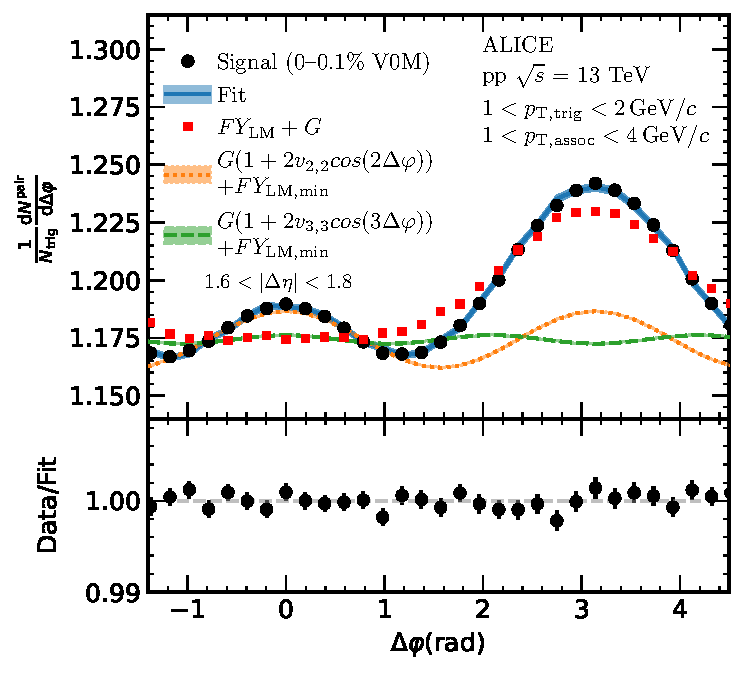
\includegraphics[width=0.6 \textwidth]{figures/Fig1_FlowExt.pdf} 
	\caption{The template fit results with the biased LM-templates. The black markers shows the signal for the $0-0.1\%$ multiplicity percentile together with its fit shown as a blue band. The red squares correspond to the LM signal. The orange and green curves correspond to the extracted $v_2$ and $v_3$ signals, respectively. The $\chi^{2}$ divided by the number of degree of freedom is 0.894}
	\label{fig:flowext}
\end{figure}

Finally, $v_{n}$ are extracted, based on the observed factorization of $v_{n,n}$ to single harmonics~\cite{ATLAS:2015hzw,ATLAS:2016yzd}, using the following equation as:
\begin{eqnarray}
v_{n}(p_{\rm{T,trig}}) = v_{n,n}(p_{\rm{T,trig}}, p_{\rm{T,assoc}}) / \sqrt{ v_{n,n}(p_{\rm{T,assoc}},p_{\rm{T,assoc}})}
\end{eqnarray}
$v_{n,n}(p_{\rm{T,assoc}},p_{\rm{T,assoc}})$ is measured in 1~$<p_{\rm{T,trig(assoc)}}<$~4~GeV/$c$ interval as the $p_{\rm{T,assoc}}$ range is fixed with 1~$<p_{\rm{T,assoc}}<$~4~GeV/$c$.

Figure~\ref{fig:flowext} shows the LM-template fit results for $0-0.1\%$ multiplicity percentile pp collisions at $\sqrt{s}$ = 13 TeV. The LM yield,  $Y_{\rm{LM}}(\Delta\varphi)$, is shown in red squares, and the extracted $v_{2}$ and $v_{3}$ as orange and green respectively. The resulting scale factor $F$ in different multiplicity percentiles and systems are summarized in Tabs.~\ref{tab:Fpp} and \ref{tab:Fpb}. They are larger for pp higher multiplicity percentiles and closer to unity for p-Pb lower multiplicity percentiles. In the previous results in Refs.~\cite{ALICE:2012eyl, ALICE:2013snk}, $F$ was assumed to be 1. The total fit is shown as a blue band and the signal to the fit is shown in the bottom panel. 
%let's add chiq value of the fit
\begin{table}[h!]
\caption{The scale factor $F$ for various multiplicity percentiles in pp collisions.}
\centering
\begin{tabular}{|c|cccc|c}
\hline
 V0M& 0--0.1\% & 1--5\% & 5--20\% & 20--60\% \\ 
 \hline
 $F$ & 1.504$\pm$0.017 & 1.414$\pm$0.030 & 1.360$\pm$0.019 & 1.208$\pm$0.015 \\  
 \hline
 \end{tabular}
 \label{tab:Fpp}
 
\end{table}

\begin{table}[h!]
\caption{The scale factor $F$ for various multiplicity percentiles in p--Pb collisions.}
\centering
\begin{tabular}{|c|cccccc|c}
 \hline
 V0A& 0--5\% & 5--10\% & 10--20\% & 0--20\% & 20--40\% & 40--60\% \\ 
 \hline
 $F$& 1.135$\pm$0.026 & 1.140$\pm$0.026 & 1.152$\pm$0.021 & 1.145$\pm$0.017 &1.092$\pm$0.015 & 1.083$\pm$0.015 \\  
 \hline
\end{tabular}
\label{tab:Fpb}
\end{table}

\begin{figure}[h!]
	\centering
	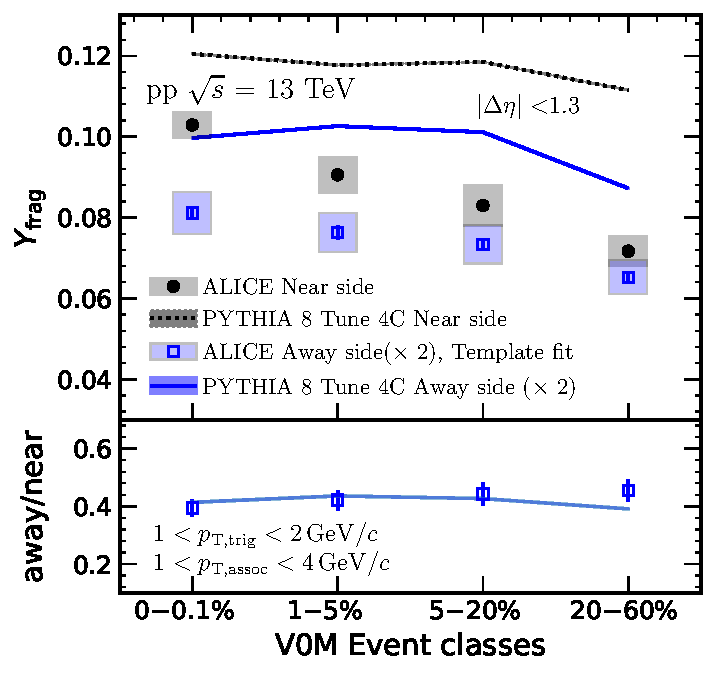
\includegraphics[width=0.6 \textwidth]{figures/Fig5_Plot_v2Mult.pdf} 
	\caption{The $Y^{\rm{frag}}$ for the near- and away-side as a function of multiplicity percentiles with both ALICE and PYTHIA data. The ratio includes the combined statistical and systematic errors in quadrature.}
	\label{fig:Ymult}
\end{figure}

\begin{eqnarray}
Y^{near}_{\rm{frag}} = \int_{|\Delta \eta|<1.3} \left( \frac{1}{\it{N}_{\rm{trig}}} \frac{ \rm{d}\it{}N_{\rm{pair}} }{ \rm{d}\Delta\eta } \right) \rm{d} \Delta\eta \quad.
\label{eq:Ynear}
\end{eqnarray}
  
The near-side jet-like yields are extracted from the near-side $\Delta\eta$ correlations, defined at $|\Delta\varphi|<$~1.3 projected on the $\Delta\eta$ axis as Eq.~\ref{eq:Ynear}. The value 1.3 is chosen as the projection range in order to fully cover $\Delta\varphi$ in Eq.~\ref{eq:pertrigger}.
The correlations in the same jet mainly contributed to $(\Delta\eta, \Delta\varphi) \sim (0,0)$ due to similar out-going direction of particles inside the jet along the jet-axis. The jet fragmentation yield is defined by integrating the $\Delta\eta$ correlation over $|\Delta\eta|<$~1.3 after applying the Zero-Yield-At-Minimum (ZYAM) procedure~\cite{Ajitanand:2005jj}. The ZYAM procedure is applied by finding the minimum value of $\Delta\eta$ correlations within $|\Delta\eta|<$1.3, which results in pointing the minimum position to be $|\Delta\varphi|=$~1.3.

The away-side jet-like yield in data is measured from the LM-template fit method as $Y^{\rm{away, HM}}_{frag} = Y^{\rm{away, LM}}_{frag} \times F$, where $F$ is again the relative contribution of the away-side jet fragmentation yield between low- and high-multiplicity events. The $Y^{\rm{away, LM}}_{frag}$ is then directly measured by integrating the away-side $\Delta\varphi$ correlation function. Since this method is not necessary for PYTHIA, where there is no flow contributions, $Y^{\rm{away}}$ is measured directly from the $\Delta\varphi$ correlation functions.

Figure~\ref{fig:Ymult} presents the $Y^{near}_{\rm{frag}}$ and $Y^{away}_{\rm{frag}}$, for both ALICE data and PYTHIA 8 Tune 4C as a function of multiplicity percentile in pp collisions at $\sqrt{s}=13$ TeV. The transverse momentum range for trigger particles is $1<p_\mathrm{T,trig}<2$ GeV/c and for associated particles $1<p_\mathrm{T,assoc}<4$ GeV/c. ALICE data points are shown as circle and square markers, whereas PYTHIA is shown as lines. The near-side yields are shown in black and the away-side yields in blue.
The near- to away-side ratio for ALICE and PYTHIA data is shown in the bottom panel. While PYTHIA overestimates ALICE data for both $Y^{near}_{\rm{frag}}$ and $Y^{away}_{\rm{frag}}$, the ratio in PYTHIA is consistent with the ALICE data in the multiplicity percentiles studied. This ratio can be explained by the pair acceptance effect caused by the limited ALICE $\eta$ acceptance~\cite{PHENIX:2006gto}, which implies that the enhanced jet yields in away-side in HM events with respect to LM events are well quantified by the LM-template method.

\subsection{Event scale dependence}
As a continuation of the extraction of the flow coefficients with the LM-template fit method, different event scale selections are investigated. By selecting events that includes a hard jet or a high-$\pt$ leading particle within the mid-rapidity region, it is possible to study the impact parameter dependence of flow coefficients in pp collisions~\cite{Sjostrand:1986ep,Frankfurt:2010ea}. This event scale is set by requiring a minimum $\pt$ of the leading track ($\ptlead$) or the reconstructed jet ($\ptjet$) at midrapidity. The leading particle track requires to be within $|\eta|<0.9$ and $0<\phi<2\pi$, and the jets are reconstructed with the anti-$k_{\rm{T}}$ algorithm~\cite{Cacciari:2008gp,Cacciari:2011ma}, with $R=$~0.4 for only charged particles. In this analysis the $\pt$ scheme is used as the recombination scheme. As the leading particle tracks, the jets are selected in the full azimuthal angle ($0<\phi<2\pi$) but in an $\eta$-range of $|\eta_\mathrm{jet}|<0.4$. The $\pt$ of jets $\ptjet$ is corrected for the underlying event density that is measured using the $k_{\rm{T}}$ algorithm with $R=$~0.2~\cite{Acharya:2018eat}.




%%%%%%%%%%%%%%%%%%%%%%%%%%%%%%%%%%%%%%%%%%%%%%%%%%%%%%%%%%

\section{Systematic uncertainties of the measured yields}
\label{sec:uncertainties}

The systematic uncertainties of $Y^{\rm{ridge}}$ and $Y^{\rm{near}}$ are estimated by varying the analysis selection criteria and corrections and are summarized in Tab.~\ref{tab:syst}.

\begin{table}[h!]
\caption{The relative systematic uncertainty of $Y^{\rm{ridge}}$ and $Y^{\rm{near}}$. Numbers given in ranges correspond to minimum and maximum uncertainties.}
\centering
\begin{tabular}{c|cc}
\hline 
\multirow{2}{*}{Sources}  & \multicolumn{2}{c}{Systematic uncertainty (\%)} \\\cline{2-3} 
         & $Y^{\rm{ridge}}$ & $Y^{\rm{near}}$ \\ \hline 
Pileup rejection    	& $\pm$0.8--3.9    &$\pm$0.2--2.2	\\ 
Primary vertex	        & $\pm$0.5--2.4	   &$\pm$1.1	\\ 
Tracking		        & $\pm$2.0--4.0    &$\pm$1.5--3.4	\\ 
ZYAM		        	& $\pm$2.1--5.1	   &$\pm$2.2--4.8	\\ 
Event mixing	    	& $\pm$1.0--4.4	   &$\pm$0.5--1.7	\\ 
Efficiency correction	& $\pm$2.5 	    &$\pm$3.1	\\  
Jet contamination   	& $-$18.8--25.9 ($\pt<$~2~GeV/$c$)	&N.A.	\\ \hline 
Total (in quadrature)			& $^{+\rm{4.9}\textrm{--}\rm{9.4}}_{-\rm{19.4}\textrm{--}\rm{21.0}}$ & $\pm$3.9--7.3 \\ 
\hline 
\end{tabular}
\label{tab:syst}
\end{table}

The systematic uncertainties are independent of the event-scale selection except for $D_{\rm{ZYAM}}$ (see below), as expected, since the multiplicity is weakly dependent on the event scale and the ALICE detector is optimized for much higher multiplicities (Pb--Pb collisions), this is in agreement with our expectations.

The uncertainty associated to the pileup rejection is estimated by measuring the changes of results with different rejection criteria from the default one. It is mainly estimated by varying the minimal number of track contributors required for reconstruction of pileup event vertices from 3 to 5. The estimated uncertainty of $Y^{\rm{ridge}}$ is 0.8-3.9\%. The corresponding uncertainty of $Y^{\rm{near}}$ is estimated to be 0.2--2.2\%.
 
Another source of systematic uncertainty is related to the selected range of the primary vertex. The accepted range is changed from $|z_\mathrm{vtx}|<$ 8 cm to $|z_\mathrm{vtx}|<$ 6 cm. The narrower primary vertex selection allows one to test acceptance effects on the measurement. The estimated uncertainty of $Y^{\rm{ridge}}$ is 0.5--2.4\%. The uncertainty for $Y^{\rm{near}}$ is estimated to be 1.1\%.

An additional source of systematic uncertainty is related to the track selection criteria. The corresponding uncertainty is estimated by employing other track selection criteria, denoted global tracks, which are optimized for particle identification. The selection criteria of the global tracks are almost identical to the hybrid tracks. Each global track is required to have at least one SPD hit. Due to inefficient parts of the SPD, the azimuthal distribution of global tracks is not uniform.
The uncertainties associated with the track selection are estimated to be 2.0--4.0\% and 1.5--3.4\% for $Y^{\rm{ridge}}$ and $Y^{\rm{near}}$, respectively.

The systematic uncertainty of $Y^{\rm{ridge}}$ resulting from the ZYAM procedure is estimated by varying the range of the fit, which is used to find the minimum, from $|\Delta\varphi|<\pi/$2 down to $|\Delta\varphi|<1.2$. The estimated uncertainty of $Y^{\rm{ridge}}$ is 2.1--5.1\%. The corresponding uncertainty on $Y^{\rm{near}}$ is estimated by varying the range from $|\Delta\eta|<$~1.6 to $|\Delta\eta|<$~1.5 and 1.7. The estimated uncertainty of $Y^{\rm{near}}$ is 2.2\% for the unbiased case and increases to 4.8\% for the largest event-scale selections. This is the only systematic uncertainty for which a significant dependence on the event scale is observed, reflecting a non-negligible dependence of the near-side magnitude and shape on the event-scale selection.

The source of systematic uncertainty is associated to the choice of the width of $z_{\rm vtx}$ bins that are used in the event mixing method. The default value of 2\,cm is changed to 1\,cm. The resulting uncertainty of $Y^{\rm{ridge}}$ is 1.0--4.4\%.
The uncertainty for $Y^{\rm{near}}$ is about 0.5--1.7\%. The uncertainty from the efficiency correction for charged particles is estimated by comparing correlation functions of true particles with correlation functions of reconstructed tracks with the efficiency correction in simulation. The estimated uncertainties are 2.5\% and 3.1\% for $Y^{\rm{ridge}}$ and $Y^{\rm{near}}$, respectively. 

In the limited $\eta$-acceptance of ALICE, the ridge structure is not flat in $\Delta\eta$ suggesting that jet-like correlations (non-flow) could contribute, implying that they would impact the ridge-yield extraction. We stress that the models used for comparisons also contain such a non-flow effect, but differences in jet-like correlations between data and MC models could influence the interpretation. To account for the related uncertainty, the variation of the yield with $\Delta\eta$ between 1.5 and 1.8, which should be an upper limit of the residual jet-like contamination, is used as a systematic uncertainty of the ridge yield. The estimated upper limit of the uncertainty is $-$25.9\% for the 1.0~$<\pt<$~1.5~GeV/$c$ range,  $-$18.8\% for the 1.5~$<\pt<$~2.0 GeV/$c$ range,  $-$18.9\% for the 1.0~$<\pt<$~2.0~GeV/$c$ range, and negligible for $\pt>$~2.0~GeV/$c$. This uncertainty is considered only for the measured ridge yields.




